\documentclass[a4paper,12pt]{article}
%%% Работа с русским языком
\usepackage[unicode, pdftex]{hyperref}
\usepackage{cmap}					% поиск в PDF
\usepackage{mathtext} 				% русские буквы в формулах
\usepackage[T2A]{fontenc}			% кодировка
\usepackage[utf8]{inputenc}			% кодировка исходного текста
\usepackage[english,russian]{babel}	% локализация и переносы
\usepackage{indentfirst}
\frenchspacing


\renewcommand{\epsilon}{\ensuremath{\varepsilon}}
\renewcommand{\phi}{\ensuremath{\varphi}}
\renewcommand{\kappa}{\ensuremath{\varkappa}}
\renewcommand{\le}{\ensuremath{\leqslant}}
\renewcommand{\leq}{\ensuremath{\leqslant}}
\renewcommand{\ge}{\ensuremath{\geqslant}}
\renewcommand{\geq}{\ensuremath{\geqslant}}
\renewcommand{\emptyset}{\varnothing}

%%% Дополнительная работа с математикой
\usepackage{amsmath,amsfonts,amssymb,amsthm,mathtools} % AMS
\usepackage{icomma} % "Умная" запятая: $0,2$ --- число, $0, 2$ --- перечисление

%% Номера формул
%\mathtoolsset{showonlyrefs=true} % Показывать номера только у тех формул, на которые есть \eqref{} в тексте.
%\usepackage{leqno} % Нумереация формул слева

%% Свои команды
\DeclareMathOperator{\sgn}{\mathop{sgn}}

%% Перенос знаков в формулах (по Львовскому)
\newcommand*{\hm}[1]{#1\nobreak\discretionary{}
	{\hbox{$\mathsurround=0pt #1$}}{}}

%%% Работа с картинками
\usepackage{graphicx}  % Для вставки рисунков
%\graphicspath{{images/}{images2/}}  % папки с картинками
\setlength\fboxsep{3pt} % Отступ рамки \fbox{} от рисунка
\setlength\fboxrule{1pt} % Толщина линий рамки \fbox{}
\usepackage{wrapfig} % Обтекание рисунков текстом

%%% Работа с таблицами
\usepackage{array,tabularx,tabulary,booktabs} % Дополнительная работа с таблицами
\usepackage{longtable}  % Длинные таблицы
\usepackage{multirow} % Слияние строк в таблице

%%% Теоремы
\theoremstyle{plain} % Это стиль по умолчанию, его можно не переопределять.
\newtheorem{theorem}{Теорема}[section]
\newtheorem{proposition}[theorem]{Утверждение}

\theoremstyle{definition} % "Определение"
\newtheorem{corollary}{Следствие}[theorem]
\newtheorem{problem}{Задача}[section]

\theoremstyle{remark} % "Примечание"
\newtheorem*{nonum}{Решение}

%%% Программирование
\usepackage{etoolbox} % логические операторы

%%% Страница
\usepackage{extsizes} % Возможность сделать 14-й шрифт
\usepackage{geometry} % Простой способ задавать поля
\geometry{top=25mm}
\geometry{bottom=35mm}
\geometry{left=25mm}
\geometry{right=20mm}
%
\usepackage{fancyhdr} % Колонтитулы
\pagestyle{fancy}
%\renewcommand{\headrulewidth}{0pt}  % Толщина линейки, отчеркивающей верхний колонтитул
% 	\lfoot{Нижний левый}
% 	\rfoot{Нижний правый}
% 	\chead{Верхний в центре}
% 	\lhead{Верхний левый}
%	\cfoot{Нижний в центре} % По умолчанию здесь номер страницы
\usepackage{lastpage}
\fancyhead[R]{АСМ. Группа Б04-004}
\fancyhead[L]{}
\fancyhead[C]{}

\usepackage{setspace} % Интерлиньяж (расстояние между строками)
%\onehalfspacing % Интерлиньяж 1.5
%\doublespacing % Интерлиньяж 2
%\singlespacing % Интерлиньяж 1

\usepackage{lastpage} % Узнать, сколько всего страниц в документе.




\usepackage[usenames,dvipsnames,svgnames,table,rgb]{xcolor}
\hypersetup{				% Гиперссылки
	unicode=true,           % русские буквы в раздела PDF
	pdftitle={Заголовок},   % Заголовок
	pdfauthor={Автор},      % Автор
	pdfsubject={Тема},      % Тема
	pdfcreator={Создатель}, % Создатель
	pdfproducer={Производитель}, % Производитель
	pdfkeywords={keyword1} {key2} {key3}, % Ключевые слова
	colorlinks=true,       	% false: ссылки в рамках; true: цветные ссылки
	linkcolor=red,          % внутренние ссылки
	citecolor=black,        % на библиографию
	filecolor=magenta,      % на файлы
	urlcolor=cyan           % на URL
}


%\usepackage[style=authoryear,maxcitenames=2,backend=biber,sorting=nty]{biblatex}

\usepackage{multicol} % Несколько колонок

\usepackage{tikz} % Работа с графикой
\usepackage{pgfplots}
\usepackage{pgfplotstable}
\usepackage{floatrow}
\DeclareFloatSeparators{mysep}{\hspace{3cm}}
\thisfloatsetup{floatrowsep=mysep}


\author{Махсудов Умар}
\title{Название работы}
\date{\today}




\newcommand{\e}[1]{
	\cdot 10^{#1}	
}

\newcommand{\s}[0]{
	\;	
}

\newcommand{\picref}[1]{
	\text{рис(\ref{#1})}
}

\begin{document}
\textbf{Цель работы:} Изучить принципы работы атомно-силового микроскопа (далее АСМ), получить и исследовать изображения решётки и CD-диска в полуконтактном режиме работы АСМ.

\textbf{Справка о сканирующей зондовой микроскопии (СЗМ)}


СЗМ относится к любым типам микроскопов, в которых изображение формируется за счёт перемещения острого зонда над исследуемой поверхностью.


Достоинства СЗМ:
\begin{itemize}
	\item
	Достоверность данных о высоте микрорельефа
	\item
	Отсутствие промежуточных процедур
	\item
	Возможность получать нанометрового и ангстремного разрешения на воздухе
\end{itemize}
\section{Принцип работы АСМ}
Диагностика поверхности с помощью АСМ основана на использовании различных видов силового взаимодействия между зондом и поверхностью. Главное преимущество атомно-силового микроскопа перед сканирующим туннельным - возможность получения с нанометровым и атомных разрешениями изображения поверхности как проводящих, так и непроводящих материалов. В случае исследования незаряженных поверхностей основной вклад в силовое взаимодействие зонда и образца дают силы силы отталкивания между ними, силы Ван-дер-Ваальса, а также капиллярные силы, связанные с наличием пленки адсорбата (воды) на поверхности образца.
\begin{figure}[H]
	\centering
	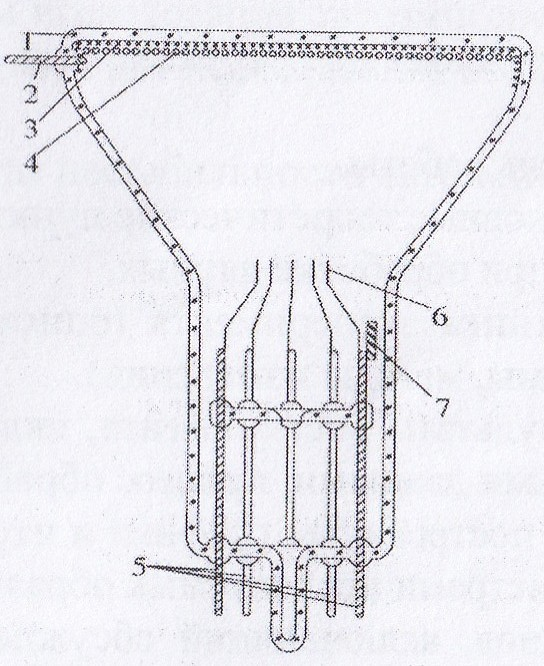
\includegraphics[scale=0.6]{pic1.jpg}
	\caption{Зависимость ван-дер-ваальсовских сил от расстояния}
	\label{pic1}
\end{figure}

Также необходимо учитывать вклад окружающей среды при измерениях. Например, капиллярные силы возникают из-за появления жидкого мостика между кончиком зонда и поверхностью (в случае ее достаточной гидрофильности).


Теоретические оценки ван-дер-ваальсовской и капиллярной силы притяжения для типичных геометрических размеров иглы: высота L = 3-15 мкм, радиус кривизны R = 5-40 нм, угол раствора конуса иглы 20-70 (градусов). Согласно этим оценкам сила притяжения по порядку величины равна:
\begin{itemize}
	\item
	$ 10^{-9}-10^{-8} $ Н для Ван-дер-Ваальсовых сил
	\item
	$ 10^{-8} Н $ для капиллярных сил. 
	
\end{itemize}

Получается, что эти силы по порядку величины совпадают с силами, характерными для межатомного взаимодействия.
Возможны 3 варианта сканирования поверхности:
\begin{enumerate}
	\item
Контактный - зонд касается поверхности
\item
Бесконтактный - на расстоянии нескольких нм
\item
Полуконтактный - зонд периодически касается поверхности
\end{enumerate}
\begin{figure}[H]
	\centering
	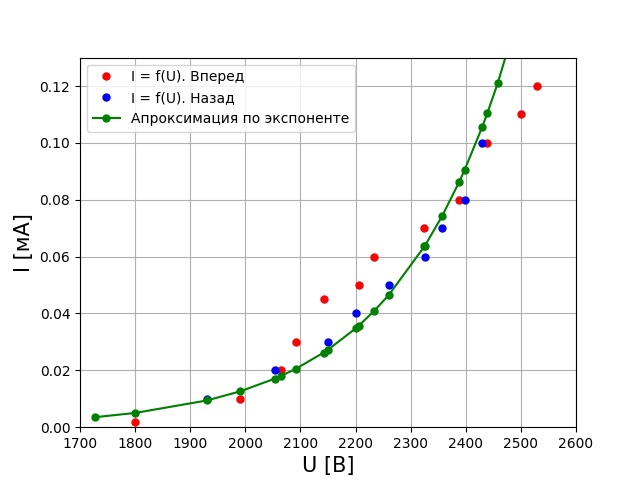
\includegraphics[scale=0.6]{pic2.jpg}
	\caption{Характеристика режимов работы}
	\label{pшс}
\end{figure}
\section{Общая схема АСМ}
Основные элементы: зонд, система регистрации отклонения зонда, пьезосканер, система обратной связи.
\begin{figure}[H]
	\centering
	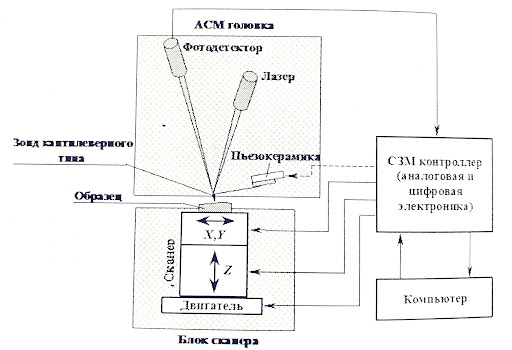
\includegraphics[scale=0.6]{pic3.jpg}
	\caption{Схема взаимодействия основных элементов АСМ (сканирование образцом)}
	\label{pic3}
\end{figure}
Пьезосканер двигает образец относительно зонда последовательно. При взаимодействии с поверхностью происходит изменение механического состояния зонда, например, отклонение кантиливера (параметр взаимодействия).
\subsection{Зонд АСМ}
В АСМ используются зонды кантеливерного типа. Кантиливер - балка с закреплённым концом. Острая игла находится на свободном конце. Кантиливер закреплён на твёрдой подложке, которая вставляется в держатель зонда, расположенный на сканере. 
\begin{figure}[H]
	\centering
	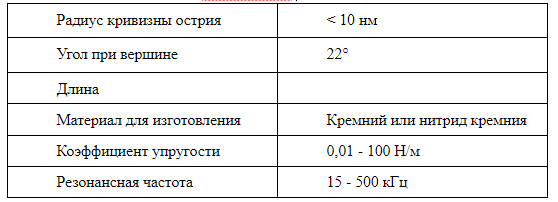
\includegraphics[scale=1]{pic4.png}
	\caption{Некоторые параметры кантеливеров}
	\label{pic4}
\end{figure}
\subsection{Измерительная головка и оптическая система регистрации отклонений кантиливера }
Измерительная головка выполняет функцию первичного преобразователя; состоит из держателя зонда и оптической системы детектирования его отклонений.


В оптической схеме регистрациии отклонений кантиливера используется метод, основанный на регистрации отклонения сфокусированного луча полупроводникового лазера ( длина волны - 670 нм, мощность - 0,9 мВт), отраженного от кончика кантиливера. 
\begin{figure}[H]
	\centering
	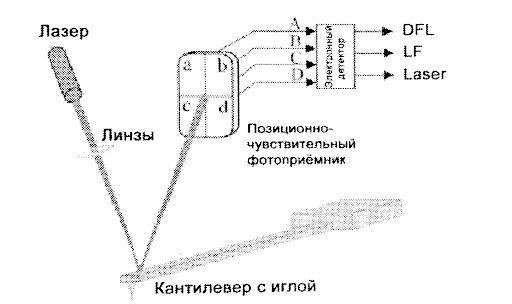
\includegraphics[scale=0.6]{pic5.jpg}
	\caption{ Оптическая схема регистрации отклонения кантиливера}
	\label{pic5}
\end{figure}
Позиционно-чувствительный фотоприемник - четырехсекционный фотодиод. Оптическая система состоит из фокусирующего объектива и зеркальной поверхности кантиливера. 


Отклонение кантиливера вызывает перемещение лазерного пятна относительно сегментов (a, b, c, d) фотодиода, что вызывает изменение электрических сигналов (A, B, C, D), поступающих с этих сегментов. Сигналы предварительно обрабатываются, и с выхода регистрирующей системы поступают 3 сигнала:
\begin{enumerate}
	\item
	DFL - сигнал, пропорциональный отклонению кантилевера в вертикальном направлении. DFL является разностным сигналом между верхней и нижней половинами фотодиода: DFL = (A+B)- (C + D). 
	\item
	LF - сигнал, пропорциональный боковому отклонению луча, который позволяет измерять крутильную деформацию кантилевера. LF является разностным сигналом между правой и левой половинами фотодиода: LF = (A + C) - (B + D). 
	\item
	LASER - сигнал, пропорциональный интенсивности света, отраженного от кантилевера. LASER является суммарным сигналом от всех четырех сегментов фотодиода: LASER = A + B + C + D. Данный сигнал используется при юстировке лазера. 
\end{enumerate}
Датчик силового взаимодействия прибора NanoEducator выполнен в виде пьезокерамической трубки длинной l=7 мм, диаметром d = 1.2 мм и толщиной h=0.25 мм, жёстко закреплённой с одного конца. Зонд имеет электрический контакт с внутренним электродом трубки, соединённым с заземлённым корпусом прибора.
\begin{figure}[H]
	\centering
	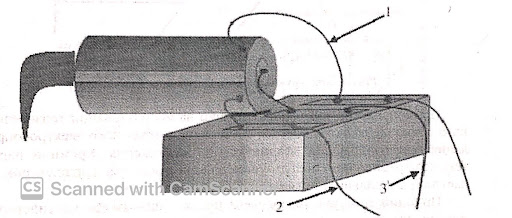
\includegraphics[scale=0.6]{pic6.jpg}
	\caption{- провод генератора, (2) - провод датчика, (3) - общий провод.}
	\label{pic6}
\end{figure}
Одна часть пьезотрубки используется как пьезовибратор, а другая - как датчик механических колебаний. к пьезовибратору подводится переменное электрическое напряжение с частотой, равной резонансной частоте силового датчика. В процессе колебаний зонда на второй части пьезоэлемента возникает переменное электрическое напряжение, пропорциональное смещению зонда, которое и измеряется прибором.
\subsection{Пьезосканер}
Сканер обеспечивает два независимых движения образца относительно кантилевера: сканирование вдоль поверхности образца (в плоскости X, Y) и перемещение в направлении, перпендикулярном к поверхности (по оси Z). Сканер изготовлен из пьезоэлектрического материала (наиболее распространенный материал - цирконат-титанат свинца), который расширяется или сжимается в зависимости от знака приложенного к нему электрического напряжения и пропорционально величине последнего. Каждый пьезосканер имеет свой уникальный пьезоэлектрический коэффициент от 0.1 до 300 нм/В. В атомно-силовых микроскопах используются различные модификации сканеров, имеющих некоторые отличия в конструкции и обеспечивающих различное максимальное поле сканирования от 3×3 $ мкм^2 $ до 100×100$  мкм^2 $. При этом максимальная измеряемая высота - от 2 мкм до 10 мкм соответственно. Большинство современных сканеров состоит из двух пьезотрубок разного диаметра, вставленных одна в другую (рис. 4). Пьезотрубка меньшего диаметра обеспечивает сканирование в плоскости образца (X,Y), большего - перемещение образца относительно кантилевера по нормали (по оси Z).
\begin{figure}[H]
	\centering
	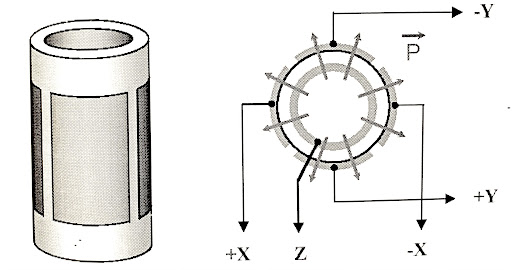
\includegraphics[scale=0.6]{pic7.jpg}
	\caption{XY-пьезотрубка сканера и схема расположения электродов XY-пьезотрубки}
	\label{pic7}
\end{figure}
Материал внутренней трубки имеет радиальное направление вектора поляризации Р. Внутренний электрод сплошной и заземлен. Вне Внешний разделен по образующим цилиндра на четыре секции. При подаче противофазных напряжений на противоположные секции внешнего электрода (относительно внутреннего) происходит сокращение участка трубки в том месте, где направление поля совпадает с направлением поляризации, и удлинение там, где они направлены в противоположные стороны. Это приводит к изгибу трубки в соответствующем направлении. Таким образом осуществляется сканирование в плоскости X, Y. Изменение потенциала внутреннего электрода внешней трубки относительно всех внешних секций приводки к удлинению или сокращению Z-трубки по оси Z.
\begin{itemize}
	\item
	Нелинейность
	
	
	Реальная пьезокерамика деформируется нелинейно с приложенным напряжением. Нелинейность обусловлена уменьшением пьезомодуля на 10-20% с ростом приложенного напряжения. 
	При получении изображений более крупных объектов, например структур, изготовленных методами микротехнологии, нелинейные эффекты могут создавать значительные искажения. Например, нелинейность XY-сканера приводит к тому, что объекты одинакового размера в начале и в конце сканируемого изображения будут иметь различные размеры.
	\item
	Гистересис 
	
	
	Это тип нелинейного поведения, при котором имеет место неоднозначная зависимость удлинения от направления изменения электрического напряжения (рис. 5). Кроме того, благодаря гистерезису керамика может не достигать своей начальной длины после одинакового изменения электрического напряжения в одну и в другую сторону.
	\begin{figure}[H]
		\centering
		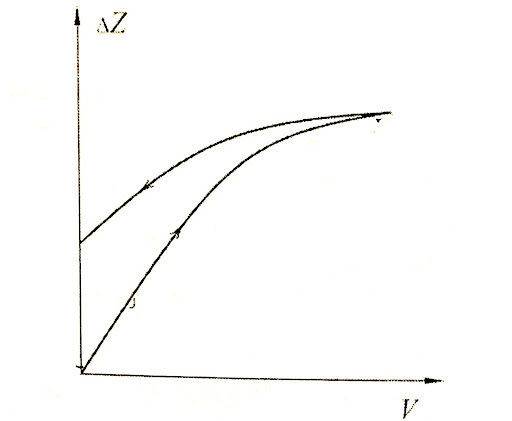
\includegraphics[scale=0.6]{pic8.jpg}
		\caption{Гистерезис пьезокерамики}
		\label{pic8}
	\end{figure}
	Величина гистерезиса обычно составляет 10\% и зависит от состава пьезоэлектрического материала и его структуры.
	Гистерезис СЗМ сканера приводит к сдвигу областей сканирования (и соответственно СЗМ-изображений), получаемых при прямом и обратном перемещениях. Поэтому для исключения искажений СЗМ-изображений поверхности образца, связанных с гистерезисом, следует проводить измерения только при прямом или только при обратном ходе сканера.
	\item 
	Ползучесть 
	
	Крип пьезокерамики проявляется в медленном дрейфе в направлении последних предшествующих перемещений или замедленном во времени механическом смещении после быстрого изменения напряжения (рис.6)
	\begin{figure}[H]
		\centering
		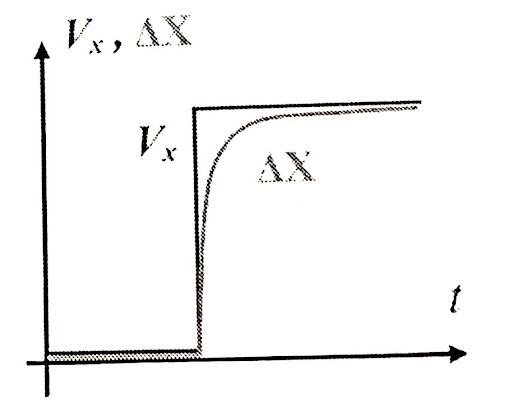
\includegraphics[scale=0.6]{pic9.jpg}
		\caption{Ползучесть и дребезг пьезокерамики}
		\label{pic9}
	\end{figure}
	Ползучесть пьезокерамики проявляется в искажении начального участка скана при больших площадях и скоростях сканирования, т.е. когда напряжение, приложенное к пьезоматериалу, изменяется достаточно быстро. Ползучесть также приводит к сдвигу особенности на СЗМ-изображении в повторных сканах. Понятно, что ползучесть проявляется при резком смещении сканера в требуемую начальную точку сканирования, поэтому в алгоритмах управления сканером исключают резкие скачки управляющего напряжения и вводят временные задержки, учитывающие ползучесть.
	\item
	Старение
	
	Коэффициент удлинения пьезоэлектрических материалов изменяется экспоненциально в зависимости от времени хранения и частоты использования. На рисунке показан график старения для часто использующегося пьезосканера и для пьезосканера, которым практически не пользуются. В тех случаях, когда сканер не используется, степень отклонения, достигаемая при определенном напряжении, постепенно снижается. Старение сканеров в АСМ может привести к понижению пьезомодуля с течением времени (рис.7). При регулярном использовании степень отклонения, достигаемая при определенном напряжении, снижается медленно.
	\begin{figure}[H]
		\centering
		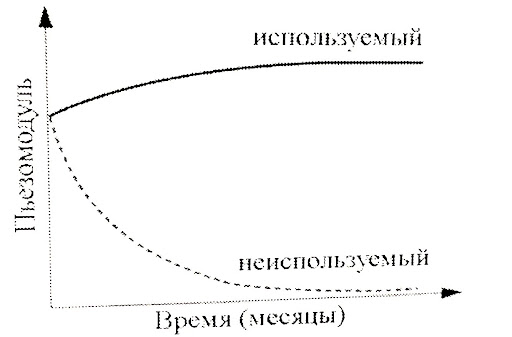
\includegraphics[scale=0.6]{pic10.jpg}
		\caption{Старение пьезокерамики}
		\label{pic10}
	\end{figure}
Таким образом, при измерении рельефа в АСМ следует иметь в виду, что значения горизонтальных (латеральных) и вертикальных размеров могут быть ошибочными, если калибровка проводилась давно.
\item
Температурный дрейф


Случайные изменения температуры, всегда существующие в лаборатории, приводят к изменению длины элементов конструкции и относительному смещению зонда и образца. 
Плавный температурный дрейф вдоль координаты Z в процессе сканирования приводит к наклону плоскости образца на СЗМ-изображении. Изменение же линейных размеров вдоль координат Х и Y, приводящее к взаимному сдвигу зонда и образца в плоскости образца, вызывает изменение масштабов изображения. В целом эти искажения похожи на искажения, вызванные ползучестью керамики. 
В современных микроскопах все больше применяются сканеры, оснащенные емкостными датчиками контроля перемещений. После калибровки с помощью оптического интерферометра либо специальных метрологических тестовых структур данные датчики позволяют судить о перемещениях образца в процессе сканирования не по напряжениям на пьезоэлементах сканера, а по фактическому смещению самого сканера. Таким образом полностью устраняется влияние гистерезиса, ползучести и теплового дрейфа пьезокерамики на результаты сканирования. Применение данных датчиков ограничено собственными шумами датчиков и разрядностью обслуживающих их систем обратной связи, поддерживающих заданное перемещение путем непрерывного подбора напряжений на пьезоэлементах сканера. Поэтому при сканировании сверхмалых объектов, а тем более при атомарном разрешении использование емкостных датчиков нецелесообразно, в связи с чем подобными датчиками оснащаются в основном сканеры с большим полем сканирования, заведомо не предназначенные для сверхвысокого разрешения.
\item
Полуконтактный режим


В режиме полуконтактной микроскопии сканирование производиться кантилевером, колеблющимся около поверхности образца. Большую часть периода колебаний кантилевер не качается поверхности и слабо взаимодействует с образцом. При соударении кантилевер теряет избыток энергии, накопленный за остальную часть периода. В зависимости от характера взаимодействия может меняться сдвиг фазы основной гармоники колебаний относительно возбуждённого сигнала, а также амплитуда и фаза высших гармоник.


Кантилевер - система с большой добротностью и высокой резонансной частотой. Лазерный луч регистрирующей системы отражается от колеблющегося в вертикальном направлении кантилевера и вызывает осциллирующее движение лазерного пятна относительно частей фотодиода. Это приводит к появлению в регистрирующей системе сигнала с частотой w. На выходе из фотодетектора сигнал DFL имеет вид $ f(t)=Asin(wt + \phi) + g(t) $, $ \phi $ - сдвиг фазы колебаний кантилевера относительно раскачивающего сигнала, g(t) - составляющая, связанная с наличием шумов и искажений. Отметим, что фаза колебаний является более чувствительной, по сравнению с амплитудой, к резким изменениям взаимодействия острия с поверхностью.


Т.к. и бесконтактный, так и полуконтактный методы являются осцилляционными методиками (кантилевер колеблется вблизи поверхности), то чрезвычайно важно понять, каким образом топография влияет на характеристики колебательной системы и что лежит в основе формирования топографического изображения.  Для начало следует сказать, что кантилевер как механическая система имеет частоту собственных колебаний $ \omega_0 $, определяемую геометрией и материалом, из которого он сделан. Для возбуждения вынужденных колебаний кантилевера микроскопы оснащаются небольшими пьезоэлементами, которые крепятся под держателем кантилевера. Этот пьезоэлемент, называемый пьезодрайвером, является преобразователем периодического электрического напряжения в периодическую механическую силу F заданной частоты $ \omega $: 

$ F(t)=F_0\cos{\Omega t} $

Под действием вынуждающей периодической силы уравнение линейных колебаний кантилевера можно записать так: 

\begin{equation}\label{key}
	\frac{d^2z}{dt^2}+2\delta\frac{dz}{dt}+\omega_0^2z=A_0\cos(\Omega t)
\end{equation}

где z(t) – отклонение кантилевера, $ А_0 $ – некоторая постоянная, а $ \delta $ – коэффициентизатухания, обусловленный неидеальностью системы. Решение этого уравнения при временах $ t \gg 1/\delta $ описывает вынужденные колебания кантилевера. Амплитуда этих колебаний $ z_0 $ и фазовый сдвиг $ \phi $ (между колебаниями вынуждающей силы и кантилевера) выражаются формулами:
\begin{equation}\label{key}
	z_0=\frac{A_0}{\sqrt{(\omega_0^2-\Omega^2)^2+4\delta^2\Omega^2}}
\end{equation}
\begin{equation}\label{key}
	\phi=arctg\frac{2\delta\Omega}{\Omega^2-\omega_0^2}
\end{equation}
Анализ выражения для амплитуды колебаний кантилевера, вынужденных
пьезодрайвером, показывает, что при вынуждающей частоте $ \Omega_k=\omega_0\sqrt{\omega_0^2-2\delta^2} $амплитуда колебаний достигает своего максимума. Эта частота называется резонансной частотой кантилевера. Вместо параметра $ \delta $ в АСМ часто используют добротность кантилевера $ Q =1/2\delta $ , которая определяет ширину резонансного пика амплитуды. Добротность зависит в первую очередь о среды измерений (вакуум, воздух), а также и от качества кантилевера. 


Теперь рассмотрим, что же произойдет, когда игла кантилевера приблизится к исследуемой поверхности на расстояние, на котором проявляется взаимодействие острия зонда и образца. Возникновение взаимодействия означает, что на образец со стороны зонда, и напротив, на зонд – со стороны образца начинает действовать сила Fзонд-образец, которая зависит от расстояния от острия до поверхности. Для описания колебаний теперь необходимо учитывать действие двух сил – периодической возбуждающей силы,  генерируемой пьезодрайвером, и силы взаимодействия зонда с поверхностью,  описываемой в первом приближении кривой на рисунке. Решение уравнение колебаний в присутствии двух сил сложнее, чем рассмотренное выше, и требует некоторых допущений, как, например, допущения о малости колебаний. Для решения Fзонд-образец раскладывается в ряд Тейлора в точке равновесия, членами выше первоготпорядка при этом пренебрегают. В результате можно показать, что появление внешней силы приводит к смещению резонансной частоты и изменению амплитуды. Изменяется и фаза колебаний.
\begin{figure}[H]
	\centering
	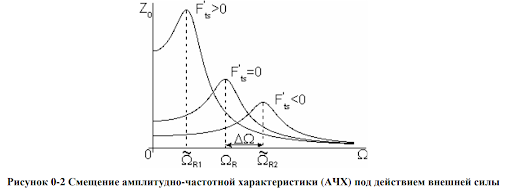
\includegraphics[scale=1]{pic11.png}
%	\caption{}
	\label{pic11}
\end{figure}
Сдвиг резонансной частоты $ \Delta\Omega $ при этом пропорционален $ dF{зонд-образец}/dz $, т.е градиенту внешней силы.
\begin{equation}\label{key}
	\Delta\Omega=\Omega_k\left( \sqrt{1-\frac{dF_{зонд-образец}}{dz}\bigg|_{z=z_0}\frac{\omega_0^2}{k\Omega^2_k}-1}\right) 
\end{equation}
где k – жесткость кантилевера, а $ z_0 $ – положение равновесия. Таким образом, изменения в резонансной частоте кантилевера могут использоваться в качестве средства измерения градиента силы, отражающего изменения в расстоянии между иглой и образцом. Если поддерживать колебания кантилевера на некоторой постоянной частоте вблизи резонанса, то смещение резонансной частоты, вызванное изменением расстояния от положения равновесия кантилевера до поверхности, приведет к изменению амплитуды колебаний кантилевера, которое может легко фиксироваться при помощи оптической системы детектирования. 
\section{Ход работы}
\begin{enumerate}
	\item
	 Включили устройство NanoEducator и запустили на компьютере рабочую программу для взаимодействия с АСМ. Установили в специальное отверстие микроскопа (1) зонд и закрепили его винтом (2), на магнитную площадку (4) установили подложку с решёткой TGT01. Закрыли микроскоп блоком с освещением и камерами (5), настроили камеры на изображение решётки (рисунок №11).
	 \begin{figure}[H]
	 	\centering
	 	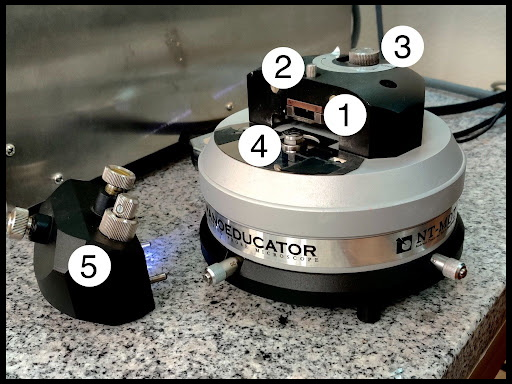
\includegraphics[scale=0.9]{pic12.jpg}
	 	\caption{Изображение установки}
	 	\label{pic12}
	 \end{figure}
	\item
	Для оценки степени остроты зонда снимем изображение установленной ранее калибровочной решёткой. Перед началом измерений в полуконтактном режиме измеряем амплитудно-частотную характеристику кантилевера (см рисунок №12)
	\begin{figure}[H]
		\centering
		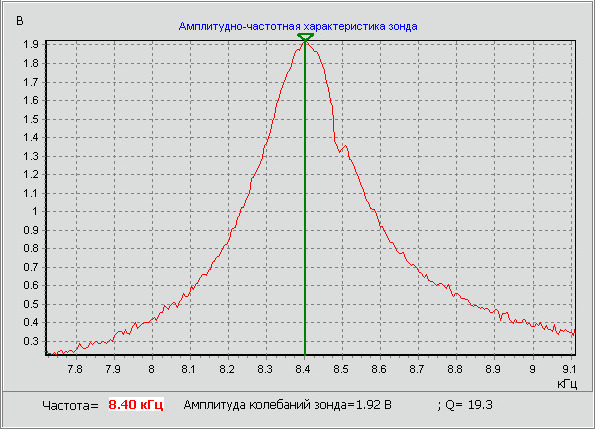
\includegraphics[scale=2]{pic13.jpg}
		\caption{АЧХ зонда}
		\label{pic13}
	\end{figure}
	Экспериментально установили, что резонансная частота кантилевера 8,40 кГц. В последующих измерениях раскачка будет производиться именно на этой частоте с амплитудой колебаний в интервале от 1 нм до 100 нм. На графике АЧХ также наблюдались более низкие пики на частотах, отличных от резонансной, что можно объяснить наличием резонансных частот у других частей утсановки (например у корпуса, или держателя канеливера).
	\item
	После осуществили подвод зонда: вручную с помощью винта (3) и с помощью программного обеспечения. После запустили программу сканирования в квадрате 10х10 микрон и шагом 50 нм. В результате получили изображение калибровочной решётки, которое обработали для дальнейшего исследования.
	\begin{figure}[H]
		\centering
		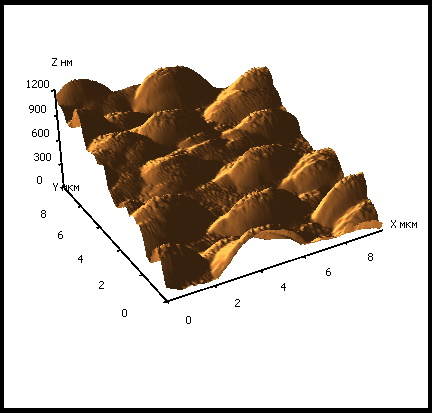
\includegraphics[scale=0.9]{pic100.jpg}
		\caption{Изометрия рельефа калибровочной решетки}
		\label{pic100}
	\end{figure}
	\item
	С помощью встроенных средств редактирования и измерения определим период решетки и её угол наклона (см рисунок №14)

	\begin{figure}[H]
		\centering
		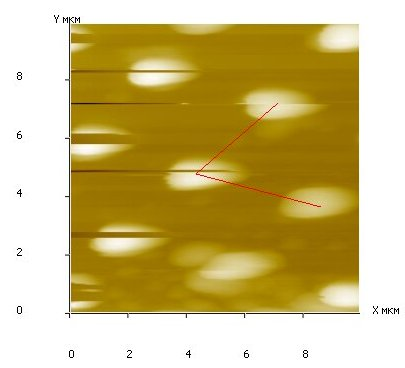
\includegraphics[scale=4]{pic102.jpg}
		\caption{Измерение периода решетки по трем пикам}
		\label{pic102}
	\end{figure}

Получены значения:
\begin{itemize}
	\item
	Период решетки: $4050 \pm 167\sнм $
	\item
	Угол решетки: $ \approx 55^\circ $
	
\end{itemize}
\item 
Зная табличные данные тестовой решетки определим радиус закругления зонда.Для этого рассмотрим продольное сечение одного из пиков решетки. Аппроксимируем скругление острия окружностью и по шкале определим ее радиус ($ \approx3.4\s мкм $).
Из геометрических соображений нетрудно установить, что $ R=(r_1+r_2) $, где $ r_1 $ - радиус острия решетки, а $ r_2 $ - радиус зонда. Из документации на решетку известно, что $ r_1\simeq 10\s нм\Rightarrow r_2\approx 1.8\s мкм $

\item
Оценив радиус острия осторожно отводим кантиливер от поверхности. Затем заменяем калибровочную решётку на образец CD-диска. Убеждаемся, что резонансна частота осталось прежней (7,85 кГц). Возвращаем зонд в рабочее положение и начинаем сканирование поверхности диска в квадрате 6х6 мкм с шагом 100 нм.
\item
Используя сечения по длине и по ширине пита определим длину, ширину и глубину пита:
\begin{itemize}
	\item
	Длина: $ 1215\pm38\s нм $
	\item
	Ширина: $ 1000\pm26\s нм $
	\item
	Глубина: $ 26\s нм $, однако, исходя из размеров зонда и размеров питы, можно сделать вывод, что зонд не сможет <<пролезть>> в углубление полность, поэтому судить о действительной глубине пита по имеющимся данным нельзя
	
\end{itemize}

\item 
Рассчитаем объем диска, если известный его геометрические размеры:
\begin{itemize}
	\item
	Внешний радиус $ R=60\s мм $
	\item 
	Внутренний радиус $ r=7.5\s мм $
	\item
	Расстояние между дорожками $ l=0.92\s мкм $
	\item 
	Ширина пита $ b=1 мкм $
	
\end{itemize}

\begin{equation}\label{key}
N=\frac{R-r}{l}\approx 57000\s дорожек	
\end{equation}
\begin{equation}\label{key}
	S=2\pi\frac{R+r}{2}N\approx1.2\e{10}\sмкм \s (Общая \sдлина \s дорожек)
\end{equation}
\begin{equation}\label{key}
	V=\frac{S}{b}\approx12\e{9}\s бит \approx 1431\s Мб
\end{equation}
Полученный результат хорошо сходится с реальным объемом CD-дика.
\item 
Далее переходим в режим “Спектрометрия”, и, выбрав относительно ровный участок на диске, получаем график (см рисунок №18). Из него находим значение для половины амплитуды $\frac{A}{2}=(86\pm11)$ нм.
\item
Отводим зонд от образца. Выключаем прибор.







\begin{figure}[H]
	\centering
	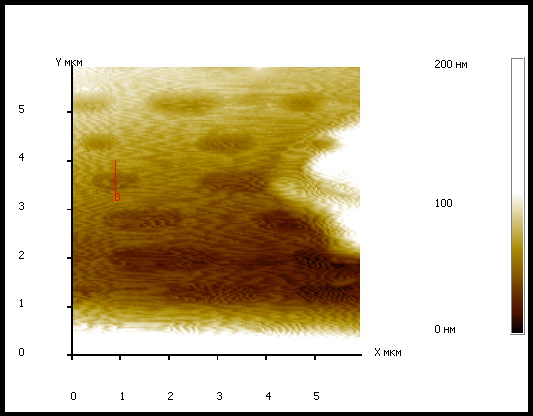
\includegraphics[scale=1]{pic106.jpg}
	\caption{Диск. Общий вид}
	\label{pшс}
\end{figure}
\begin{figure}[H]
	\centering
	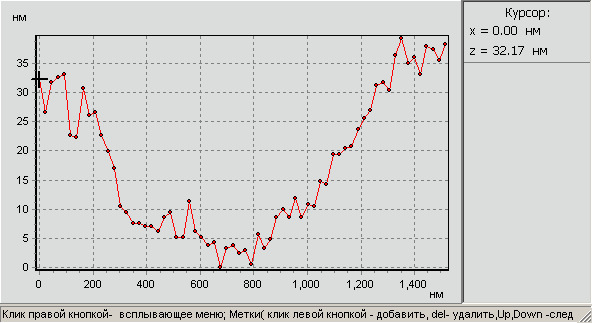
\includegraphics[scale=0.7]{pic104.jpg}
	\caption{Диск. Сечение по длине пика}
	\label{pшс}
\end{figure}
\begin{figure}[H]
	\centering
	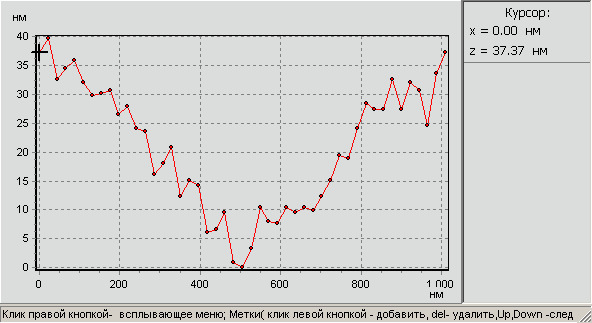
\includegraphics[scale=0.7]{pic105.jpg}
	\caption{Диск. Сечение по ширине пика}
	\label{pшс}
\end{figure}
\begin{figure}[H]
	\centering
	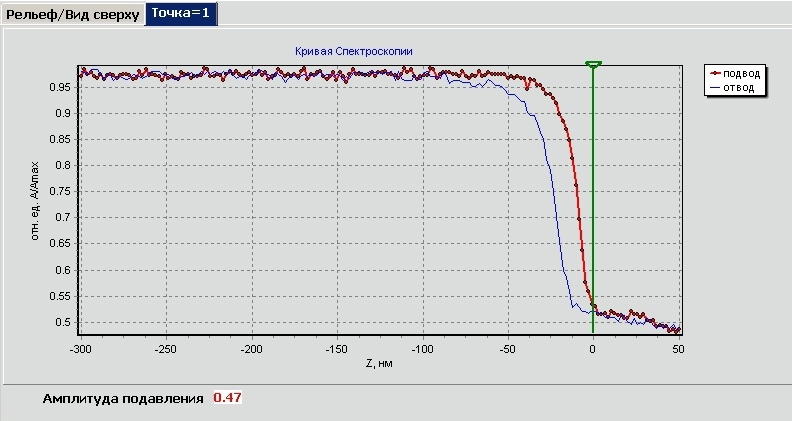
\includegraphics[scale=2]{fin.jpg}
	\caption{Спектрограмма}
	\label{pшс}
\end{figure}


	
\end{enumerate}
\section{Выводы}
В данной работе мы познакомились атомно-силовым микроскопом с теоретической и практической точки зрения. Изучили основной принцип работы, режимы измерений, достоинства и недостатки основных методов микроскопии. В практической части нам удалось получить сканы двух образцов: тестовой решетки, с помощью которой была определен радиус закругления зонда и участок CD-диска. Все измеренные параметры поверхности CD-диска, за исключением глубины пика, в пределах $\sigma$ совпали со значениями, предусмотренными стандартом.



         

 


\end{itemize}








	
\end{document}
